\section{Evaluation}
\label{sec:eval}
In this section, we introduce the dataset, 
baselines and experimental setup.
We show the results and analyze 
the performance of our model~\footnote{
All datasets, source code and generated summaries
can be downloaded from
http://202.120.38.146/sumrep.}.


\subsection{Datasets}
CNN/Daily Mail dataset~\cite{HermannKGEKSB15,NallapatiZSGX16,SeeLM17}
\footnote{\url{https://cs.nyu.edu/~kcho/DMQA/}} is a popular 
summarization dataset, 
which contains news articles paired with summaries.
There are 286,817 training pairs,
13,368 validation pairs and 11,487 test pairs.
%\tabref{table:cnn} shows an example pair from training data.
We follow See~\shortcite{SeeLM17} in data preprocessing and use 
the non-anonymized version. 
%fill in the blanks with answer named entities.
%We show an example of such pairs in \tabref{tab:gold_a}.

\subsection{Baselines}
We introduce the baselines involved in our experiments.
For fair comparison, we construct several baselines 
(\tabref{tab:baselines}) by converting some of RNN-based models to
CNN seq2seq architectures. Details are illustrated in \secref{sec:related}.
%since most works in summarization are RNN-based. 
\begin{table}[th]
	\centering
	\scriptsize
	\begin{tabular}{|l|l|}
		\hline
		\textbf{Abbrev.} & \textbf{Description} \\ \hline
		\textbf{CNN} &  Convolutional seq2seq model~\cite{gehring2017convs2s} \\
		\hline
		\textbf{ITA} &  Intra-temporal attention~\cite{NallapatiZSGX16} \\
		\hline
		\textbf{ITDA} & \tabincell{l}{Intra-temporal attention and intra-decoder attention\\ \cite{PaulusXS17,FanGA18}}\\
		\hline
	    \textbf{COV}	& Coverage mechanism~\cite{SeeLM17}\\
		\hline
        \textbf{TRI} & Trigram decoder~\cite{PaulusXS17} \\
		\hline
	\end{tabular}
	\caption{Baselines}
	\label{tab:baselines}
\end{table}

\cut{%%%%%%%%%%%%
\itemsep0em
\begin{itemize}
\item \textbf{CNN} is the original convolutional seq2seq model \cite{gehring2017convs2s}. 
\item \textbf{COV} adopts the coverage mechanism \cite{SeeLM17}, where repeatedly
attending to the same locations is penalized in the form of \textit{coverage loss}. 
\item \textbf{ITA} integrates \textit{intra-temporal attention} \cite{NallapatiZSGX16} in CNN seq2seq model, which normalizes attention values using attention history through time stamps. 
\item \textbf{ITDA} adds \textit{intra-decoder attention} mechanism \cite{PaulusXS17} based on ITA,
which also normalizes attention values using past decoders states.
It is transferred to CNN seq2seq model in \cite{FanGA18}.
\item \textbf{TRI} uses \textit{trigram decoder} \cite{PaulusXS17} at testing. The generation of repetitive trigrams is banned during beam search.
\end{itemize}
}%%%%%%%
%\textbf{CNN} stands for the original convolutional seq2seq model from \cite{gehring2017convs2s}. Next, we borrow the coverage mechanism from \cite{SeeLM17} to build our \textbf{COV} model as another baseline, where repeatedly
%attending to the same locations is penalized in the form of \textit{coverage loss}. In \textbf{ITA}, we incorporate \textit{intra-temporal attention} from \cite{PaulusXS17} into convolutional seq2seq model, which normalizes attention scores using attention history through timestamps. In \textbf{ITDA} model, we further add \textit{intra-decoder attention} mechanism \cite{PaulusXS17}, which normalizes attention using past decoders states. \textbf{TRI} revises beam search in test time in the same way as mentioned in section 2.5 of \cite{PaulusXS17}. In this model, generation of repetitive trigrams is banned during beam search in hope of reducing repetition.

\subsection{Experimental Setup}
\label{sec:expset}
In the following, 
all the competing models contain $8$ convolutional layers in
both encoders and decoders, with kernel width of $3$.
For each convolutional layer, 
we set the hidden state size to $512$ and the embedding size to $256$.
To alleviate overfitting,
we apply a \textit{dropout} ($p=0.2$) layer to 
all convolutional and fully connected layers.

%To optimize our proposed model,
We use Nesterov's
accelerated gradient method \cite{SutskeverMDH13} with gradient clipping $0.1$ \cite{PascanuMB13}, momentum $0.99$,
and initial learning rate $0.2$.
Training terminates when learning rate $\le 10e$-$5$.
Beam size $b=5$ at test time.

%To obtain our model with attention filter mechanism and 
%sentence-level backtracking decoder, we set
%set size $sz$ (\secref{sec:attf}) to $3$.
We set the threshold $sz$ (\secref{sec:attf}) to $3$, 
because nearly $90\%$ 
of sections are with length$>=$3.
We set $n$ (Equation (\ref{eq:s})) to $5$,
%since the numbers of overlapped words in most reference summaries 
%are less than $5\%$.
since less than $5\%$ of reference summaries have
the longest common substring (LCS) of less than $5$.
We use the following evaluation metrics:
\itemsep0em
\begin{itemize}

\item \textbf{ROUGE} scores (F1), including ROUGE-1 (R-1), ROUGE-2 (R-2) and
ROUGE-L(R-L)~\cite{rouge-a-package-for-automatic-evaluation-of-summaries}.
%ROUGE-2 is the most popular metric for summarization.

\item \textbf{Repeatedness} (Rep) includes N-gram repeatedness, sentence repeatedness
and total repeatedness. 
N-gram or sentence repeatedness is the percentage of repeated N-grams 
or sentences in a summary:
%For a sentence, we get $sim$ between it and other sentences
%in the same summary. If $sim=1$, it is repeated.
%Both repeated N-grams and sentences are repeated units.

\begin{equation}
\small Rep = \frac{n}{N}
\end{equation}
where $n$ is the number of repeated N-grams or sentences, 
$N$ is the total number of N-grams or sentences in a summary.
We use \textit{sim} in \eqnref{eq:s} to %estimate
%whether an N-gram or a sentence repeats.
determine whether there is sentence repetition.
Total repeatedness (Algorithm \ref{alg:red}) is a comprehensive score that unifies N-gram and sentence repeatedness.
%It is caused by repetitve substring in a summary.
%The calculation of total repeatedness is illustrated in 
%Algorithm \ref{alg:red}.
%\item \textbf{Redundancy} (Red) is caused by
%repetitive substrings in a summary. 
%Being \textit{repetitive} means the same sequence appears more than once in a summary. 
%Here we only focus on \textit{repetitive} substrings containing more than two words.
%The calculation of redundancy is illustrated in Algorithm \ref{alg:red}.
%Redundancy is a comprehensive score that unifies N-gram and sentence repeatedness.
%Redundancy is different from repeatedness in that it takes into account the length and the number of appearance of repetitive substrings in summary. 
%\KZ{Revise algo 1. I think it can be simplified.}
\begin{algorithm}[th]
\caption{Calculation of Total Repeatedness}
\scriptsize
\label{alg:red}
\textbf{Input}: a sentence set $s = {s_{1}, s_{2},...,s_{n}}$\\
%\textbf{Parameter}: Optional list of parameters\\
\textbf{Output}: Total repeatedness percentage $p$
\begin{algorithmic}[1] %[1] enables line numbers
\STATE Let $total$ be the sum of lengths of the sentences in $s$.
\STATE $n \leftarrow total$
\STATE $overlap \leftarrow 0$
\WHILE{$n \geq 3$}
\STATE The lengths of longest common substring (LCS) between two sentences from $s$ comprise a length set, $len\_set$.
\STATE $n \leftarrow \max(len\_set)$.
\STATE Find a substring $b$ with length $n$ that appears most frequently in $s$.
\STATE Let $k$ be the frequency that $b$ appears in $s$.
\STATE $overlap \leftarrow overlap + k\cdot n$
\STATE Remove every appearance of substring $b$ from sentences in $s$.
\ENDWHILE
\STATE $p \leftarrow overlap/total$
\STATE \textbf{return $p$} 
\end{algorithmic}
\end{algorithm}

\item \textbf{Readability} (Readable) is a kind of human evaluation, 
the percentage of
\textit{readable} sentences in generated summaries.
%Sentences are more complete than segment so that they can
%be evaluated easily.
Here we score sentences instead of segments because segments often have
insufficient information to determine readability.
A \textit{readable} sentence is free of grammatical and 
factual errors, 
and is logically consistent with source document.
%\begin{equation}
%Correct = \frac{n_{ct}}{N_{all}}
%\end{equation}
%where $n_{ct}$ and $N_{all}$ denotes
%the number of \textit{correct} sentences and all sentences 
%in a summary respectively.
\end{itemize}

We use \textit{readability} to complement ROUGE scores 
since Yao~\shortcite{Yao} showed that the standard 
ROUGE scores cannot capture grammatical or factual errors. 
We randomly sample 300 summaries generated by each model
and manually check their readability. 
%This is a simplified human-evaluation of summarization,  
%It is easier to do and more reliable than other human-evaluations
%since we only need to check whether the sentences in a summary are \textit{correct} or not.
This metric is more objective and practical compared with
scoring the whole summary \cite{D18-1205}, since we only need 
to determine whether a sentence is {\em readable} or not.
Each sentence is scored by two judges proficient in English. 
The Cohen's Kappa coefficient between them is $0.83$, 
indicating agreement. Here we use the average annotation score.
%The score of each model is the proportion
%of {\em readable} sentences in total.

\subsection{Results}
\label{sec:result}

\textbf{Accuracy.} As shown in \tabref{tab:eval_main}, 
our proposed model (ATTF+SBD)
outperforms all the baselines in ROUGE score, indicating we are able to generate more
accurate summaries. Without any special operations at test time, our attention
mechanism ATTF achieves the highest ROUGE score, demonstrating
its efficacy in improving summary quality.
%ATTF is effective to improve the summarization quality of basic CNN seq2seq models.

Models with SBD or TRI at testing time
are more effective than the basic CNN seq2seq model,
%This is due to more information involved in the generation 
because more information is involved in summary generation 
as a by-product of repetition reduction.
%Both SBD and TRI gain great improvements in ROUGE score, 
%\XS{need to rephrase the following sentence.} 
%due to the model is able to select other candidate words,
%which are adjust to reference summary, after reducing repetition. 
%SBD-b1 and SBD-b2 are baselines of SBD.
Compared with its two variants, SBD is a little slower 
%\XS{lower of what?}
but has a higher ROUGE score, reflecting its advantage due to
better choices taken globally.
%\XS{need to rephrase the following sentences.} 
%because generation of sentences in summary is not disturbed using SBD. 
Therefore, 
we use SBD as our backtracking decoder in the following experiments. 
The number of explored candidate hypothesis, up to a point of
repetition, is less than 30 tokens.
The ROUGE score of SBD is higher than TRI on R-1 and R-L, but lower on R-2. 
The reason is that R-2 and R-L respectively evaluate
bigram-overlap and longest common sequence between the reference
summary and generated summary. This is in line with different techniques 
in SBD and TRI, the former promoting the diversity of sentences and 
the latter promoting that of trigrams.

%Corresponding to this,
%SBD select words
%on sentence level while TRI is based on trigrams.
%Comparing ATTF+SBD and ATTF+TRI, ATTF+SBD is better.
For models that tackle repetition both at train-time and test-time, 
ATTF+SBD outperforms ATTF+TRI.
SBD works in synergy with ATTF, both of which process 
information with \textit{section/segment} as a unit.
%Because ATTF filters attention scores between summary and source document
%by each segment in summary, and it needs sentence level 
%information more than 
%n-gram information. 
%Besides, the ROUGE scores of ATTF+SBD are not better than
%those reported in \cite{SeeLM17,PaulusXS17,FanGA18}. 
The ROUGE scores of ATTF+SBD do not surpass
those reported in \cite{SeeLM17,PaulusXS17,FanGA18}. 
%Because reducing repetition is a part of 
%their summarization task.
Their improvement is not entirely
due to repetition reduction 
as they apply other methods to enhance ROUGE scores 
in different aspects. 
We aim to estimate the models' ability of
reducing repetition in summarization alone,
so we implement their repetition reduction methods 
on CNN seq2seq model. Our ATTF+SBD model 
scores higher in ROUGE scores than the other baselines, 
demonstrating that it can more properly reduce 
repetition and generate more accurate summaries.

\begin{table}[th]
	\centering
	\scriptsize
	\begin{tabular}{|l|c|c|c|}
		\hline
		Model &   R-1 & R-2 & R-L \\
		\hline
		CNN &  34.34 & 14.25 & 25.68 \\
		ITA &  34.30 & 14.20 & 25.67 \\
		ITDA & 34.53 & 14.41 &  25.81 \\
	    COV	& 35.85 & 14.80 &  25.95 \\
        TRI* & 36.81 & 15.47 & 26.00 \\
		\hline
		SBD-b1* & 34.24 & 14.33 & 24.75 \\
		SBD-b2* & 35.88 & 14.83 & 25.15 \\
		SBD* & 37.19 & 15.45 & 26.03 \\
		ATTF & 36.32 & 15.08 & 26.09 \\
		ATTF+TRI* & 37.33 & 15.65 & 26.30 \\
		ATTF+SBD* & \bf 37.69 & \bf 15.82 & \bf 26.47 \\
		\hline
	\end{tabular}
	\caption{ROUGE scores on CNN/Daily Mail dataset. `*' denotes 
models with operations during testing.}
	\label{tab:eval_main}
\end{table}

\textbf{Repeatedness.}
To demonstrate the effectiveness of ATTF and SBD in reducing repetition, 
we compare \textit{repeatedness} (\tabref{tab:eval_repe}) 
of generated summaries.
%The lower repeatedness reflects larger ability of reducing repetition.
Lower repeatedness 
means the model is more capable of reducing repetition.

\begin{table*}[th]
	\centering
	\scriptsize
	\begin{tabular}{|c|c|ccccc|cccc|}
		\hline
	            & Gold & CNN  & ITA & ITDA & COV & ATTF & TRI* & SBD* & ATTF+TRI* & ATTF+SBD* \\
		\hline
		1-gram & 33.79 & 56.25 & 54.44 & 51.18 & 42.18 & \bf 34.98 & 31.91 & \bf 29.88 & 32.0 & 30.83 \\
		2-gram & 2.98 & 36.55 & 34.76 & 30.64 & 16.77 & \bf 8.16 & 3.17 & \bf 2.84 & 2.94 & 3.71 \\
		3-gram & 0.43 & 32.62 & 31.10 & 27.14 & 12.95 & \bf 5.11 & \bf 0.0 & 0.40 & \bf 0.0 & 0.74 \\
		4-gram & 0.12 & 30.18 & 28.85 & 25.04 & 11.17 & \bf 4.19 & \bf 0.0 & 0.06 & \bf 0.0 & 0.13 \\
		Sent & 0.08 & 37.04 & 35.79 & 31.46 & 13.98 & \bf 3.56 & \bf 0.0 & \bf 0.0 & \bf 0.0 & \bf 0.0 \\
		\hline
		Total-Rep & 0.51 & 18.86 & 17.94 & 15.62 & 16.46 & \bf 3.27 & \bf 0.0 & 0.44 & \bf 0.0 & 0.80 \\
		\hline
		Readable & 1.0 & 0.65 & 0.75 & 0.76 & 0.80 & \bf 0.86 & 0.75 & 0.85 & 0.77 & \bf 0.93 \\
		\hline
	\end{tabular}
	\caption{Repeatedness scores (\%) and Readability scores on CNN/Daily Mail dataset.}
	\label{tab:eval_repe}
\end{table*}

\cut{%%%%%%%%%%%%%%%
\begin{table}[th]
	\centering
	\scriptsize
	\begin{tabular}{|l|c|c|c|c|c|c|c|}
		\hline
		Model & 1-gram  & 2-gram & 3-gram & 4-gram & sent \\
		\hline
		Gold & 33.79 & 2.98 & 0.43 & 0.12 & 0.08 \\
		\hline
		CNN &  56.25 & 36.55 & 32.62 & 30.18 & 37.04  \\
		ITA & 54.44 & 34.76 &31.10 & 28.85 & 35.79 \\
		ITDA & 51.18 & 30.64 & 27.14 & 25.04 & 31.46 \\
		COV & 42.18 & 16.77 & 12.95 & 11.17 & 13.98  \\
		ATTF & \bf 34.98 & \bf 8.16 & \bf 5.11 & \bf 4.19 & \bf 3.56 \\
        \hline
		TRI* & 31.91 & 3.17 & \bf 0.0 & \bf 0.0 & \bf 0.0 \\
		SBD* & \bf 29.88 & \bf 2.84 & 0.40 & 0.06 & \bf 0.0 \\
		\tiny ATTF+TRI* & 32.0 & 2.94 & \bf 0.0 & \bf 0.0 & \bf 0.0 \\
		\tiny ATTF+SBD* & 30.83 & 3.71 & 0.74 & 0.13 & \bf 0.0 \\
		\hline
	\end{tabular}
	\caption{Repeatedness scores (\%) on CNN/Daily Mail dataset. `*' denotes models with operations at testing.}
	\label{tab:eval_repe}
\end{table}
}%%%%%

In \tabref{tab:eval_repe}, Gold row shows the repeatedness scores of
reference summaries. ATTF achieves the lowest
score among all baselines without any operations at test time. 
%It denotes that our model has ability to remember 
%the summarized part of source document by segments in summary.  
%Compared with summaries generated by 
\figref{fig:attn_maps} shows that baseline models 
suffer from severe repetition problem because they attend to the same POIs 
of the source document, whereas 
ATTF attends to different POIs and generates summaries 
such as this:

\fbox{
\parbox{0.9\columnwidth}{
\small{\textbf{ATTF}: ``manchester city are rivalling manchester united and arsenal for defender dayot 
pamecano . the 16-year-old joined in the january transfer window only for 
him to opt to stay in france . ''
}}}

\begin{figure}[th!]
\centering
\subfigure[COV]{
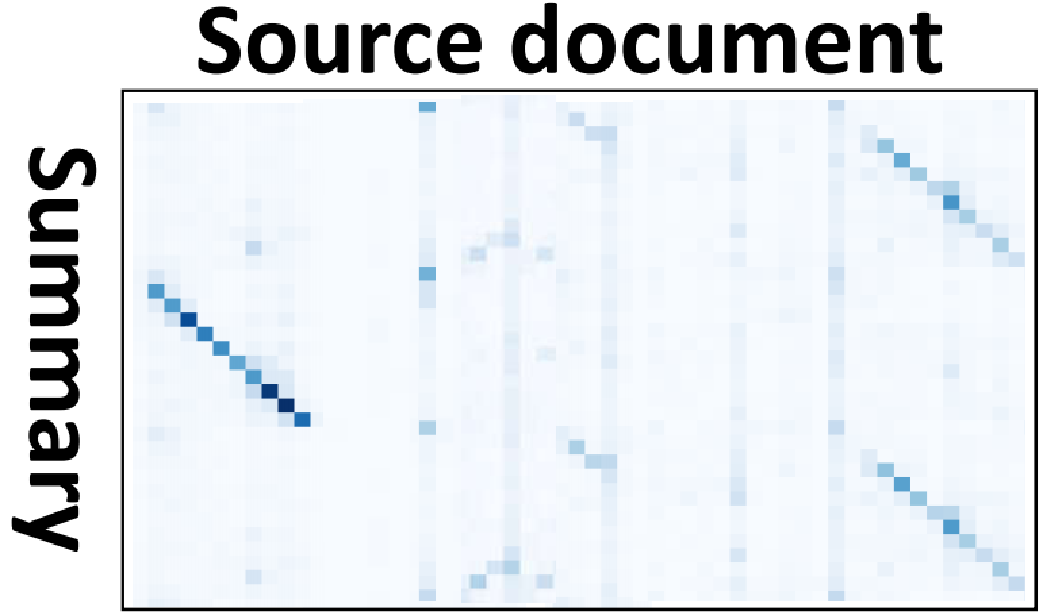
\includegraphics[width=0.4\linewidth]{mapCOV}
}
\quad
\subfigure[ITA]{
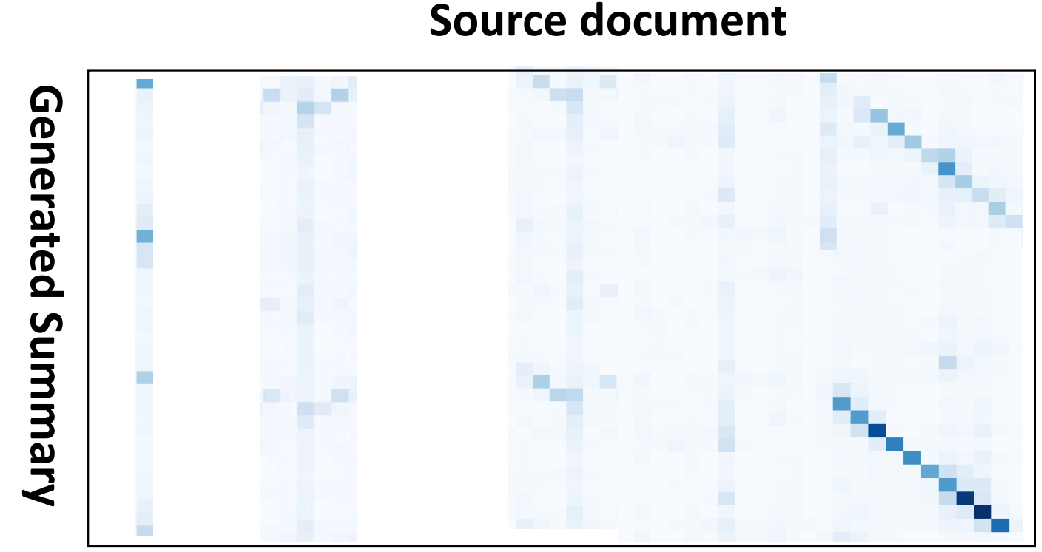
\includegraphics[width=0.4\linewidth]{mapITA}
}
\quad
\subfigure[ITDA]{
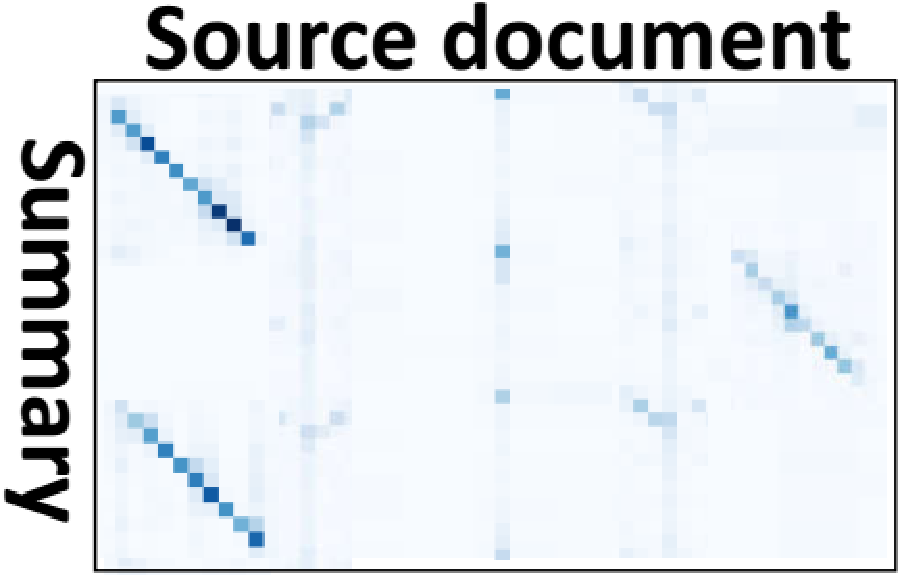
\includegraphics[width=0.4\linewidth]{mapITDA}
}
\quad
\subfigure[ATTF]{
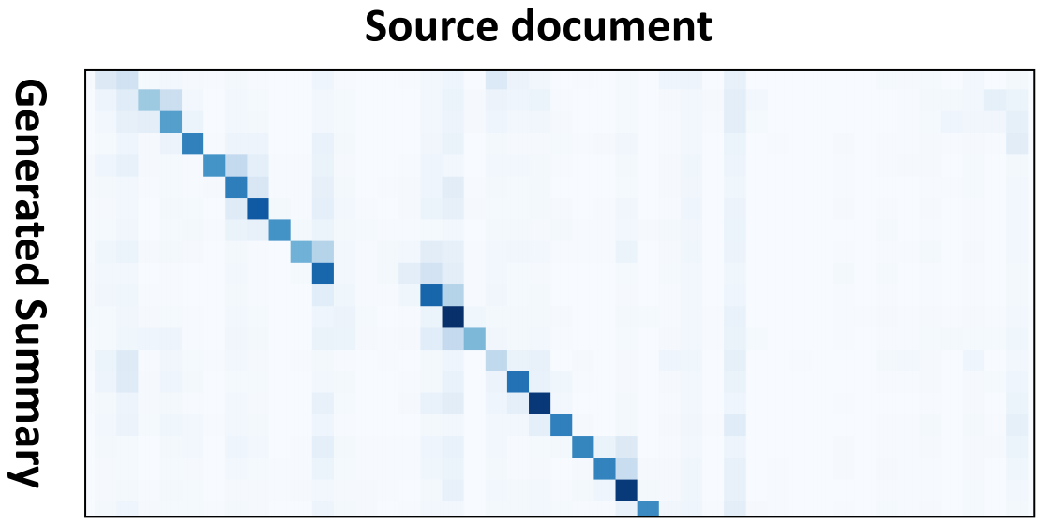
\includegraphics[width=0.4\linewidth]{map2}
}
\caption{Attention distribution of examples in \tabref{tab:strong_methods}}
\label{fig:attn_maps}
\end{figure}

Compared with the Gold standard,
ATTF still generates some repetitive sentences,
due to similar sentences in the source document
such as \exref{ex:repeatsrc}.
%The result of summarizing that document using ATTF and its local attention map are
The summary generated by ATTF and its local attention are
shown in \tabref{tab:src_rep} and \figref{fig:attn_map3}.
Also, SBD further reduces the repetition when combined with ATTF. 
%which demonstrates its effectiveness.

\begin{table}[th!]
\begin{center}
\scriptsize
\begin{tabular}{|l|}%{|p{7cm}|rl|}
%\hline \bf Source document \\
%\hline chelsea 's on loan midfielder oriol romeu goes up against sportsmail 's \\
%       martin ... . the standout fixture in the league on saturday sees leaders \\
%	   chelsea welcome manchester united to stamford bridge , ... \\
%	   chelsea midfielder oriol romeu , \textbf{currently on loan at stuttgart} , predicts \\
%	   the scores for the weekend 's matches . romeu is \textbf{currently on a season-long} \\
%	   \textbf{loan at bundesliga side stuttgart .} \\
%\hline \bf Reference summary \\
%\hline oriol romeu is on a season-long loan at stuttgart from chelsea . the spanish \\
%       midfielder predicts the scores in saturday 's matches . romeu goes \\
%	   head-to-head with sportsmail 's martin keown . \\
\hline \bf Our(Attention Filter)\\
\hline chelsea beat manchester united on saturday . \textit{oriol romeu is currently} \\
       \textit{on a season-long loan at stuttgart . oriol romeu is} \\
	   \textit{currently on a season-long loan at bundesliga side stuttgart .}\\
\hline \bf Our(Attention Filter + Backtracking decoder) \\
\hline chelsea face manchester united in the premier league on saturday . oriol \\
       romeu is currently on loan at stuttgart . \\
\hline
\end{tabular}
\end{center}
\caption{Summaries generated from \exref{ex:repeatsrc}.}
\label{tab:src_rep}
\end{table}


\begin{figure}[th!]
\centering
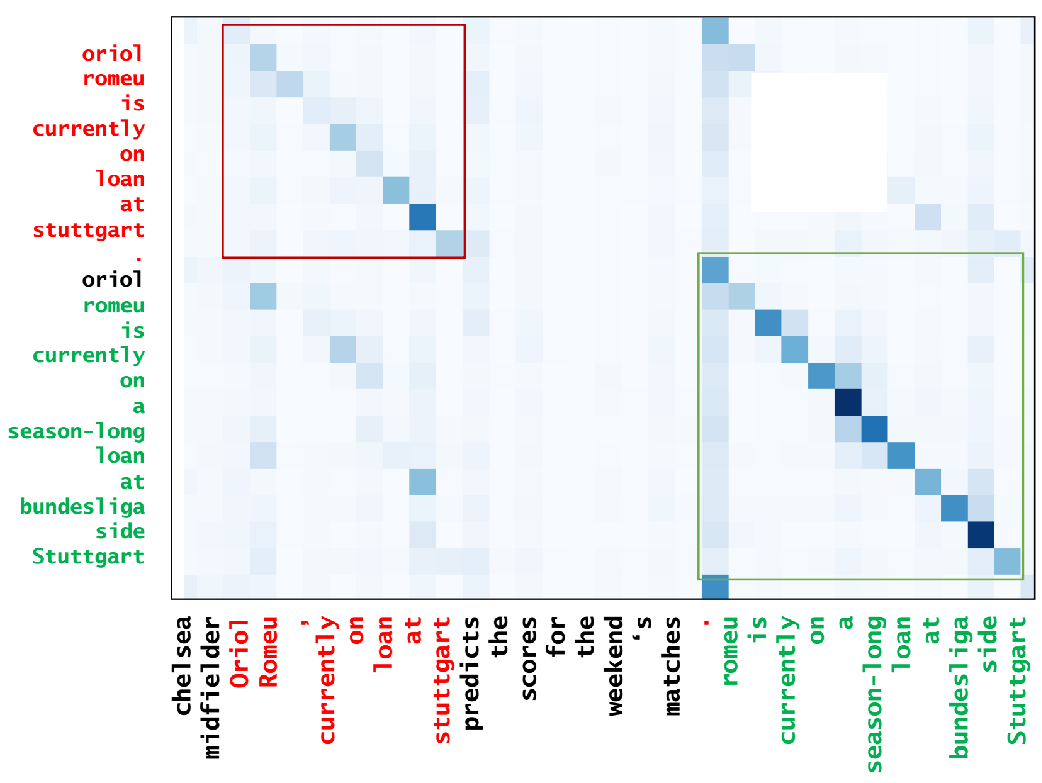
\includegraphics[width=0.8\linewidth]{map3}
\caption{Attention distribution for ATTF in \tabref{tab:src_rep}}
\label{fig:attn_map3}
\end{figure}


%The repeatedness of models with TRI is the lowest among all of the models, 
%\KZ{Compared with SBD and ATTF+SBD, I don't think TRI is that much better
%in repeatness score. In fact it's larger in repeatness scoreon 1-gram
%and 2-gram. Then what do you mean by ``remarkable''?}
As shown in \tabref{tab:eval_repe}, TRI has the lowest total repeatedness score.
%which means that 
%It does not generate any
%repetitive N-grams (N$>$2) and sentences. Because TRI
%prevents the generation of the same trigrams during testing.
It does not generate any repetitive N-grams (N$>$2) and sentences 
because TRI prevents the generation of the same trigrams during testing.
But as the Gold row shows, reference summaries do have some natural repetition.
%As reference summaries are human written, 
Therefore we evaluate the correlation of repeatedness distribution between
generated summaries and reference summaries (\tabref{tab:eval_repcor}).
Our proposed models achieve better results, among which ATTF+SBD performs best, an indication that ATTF and SBD are more capable of producing summaries with a natural level of repeatedness.
%It indicates that ATTF and SBD are more capable of producing summaries with a natural level of repeatedness.
%missing POIs and repetition in source documents.

\begin{table}[th]
	\centering
	\scriptsize
	\begin{tabular}{|l|c|c|c|}
		\hline
		     & pearson  & spearman & kendall's tau \\
		\hline
		TRI* & 1.0 & 0.894 & 0.837  \\
		SBD* & 1.0 & 1.0 & 1.0 \\
		%ATTF & 0.998 & 0.943 & 0.867 \\
		ATTF+TRI* & 1.0 & 0.894 & 0.837 \\
		ATTF+SBD* & \bf 1.0 & \bf 1.0 & \bf 1.0 \\
		\hline
	\end{tabular}
    \caption{Repeatedness correlation between generated summaries and Gold summaries.}
	\label{tab:eval_repcor}
\end{table}
	
	
\cut{%%%%%%%%
\begin{figure}[th!]
\centering
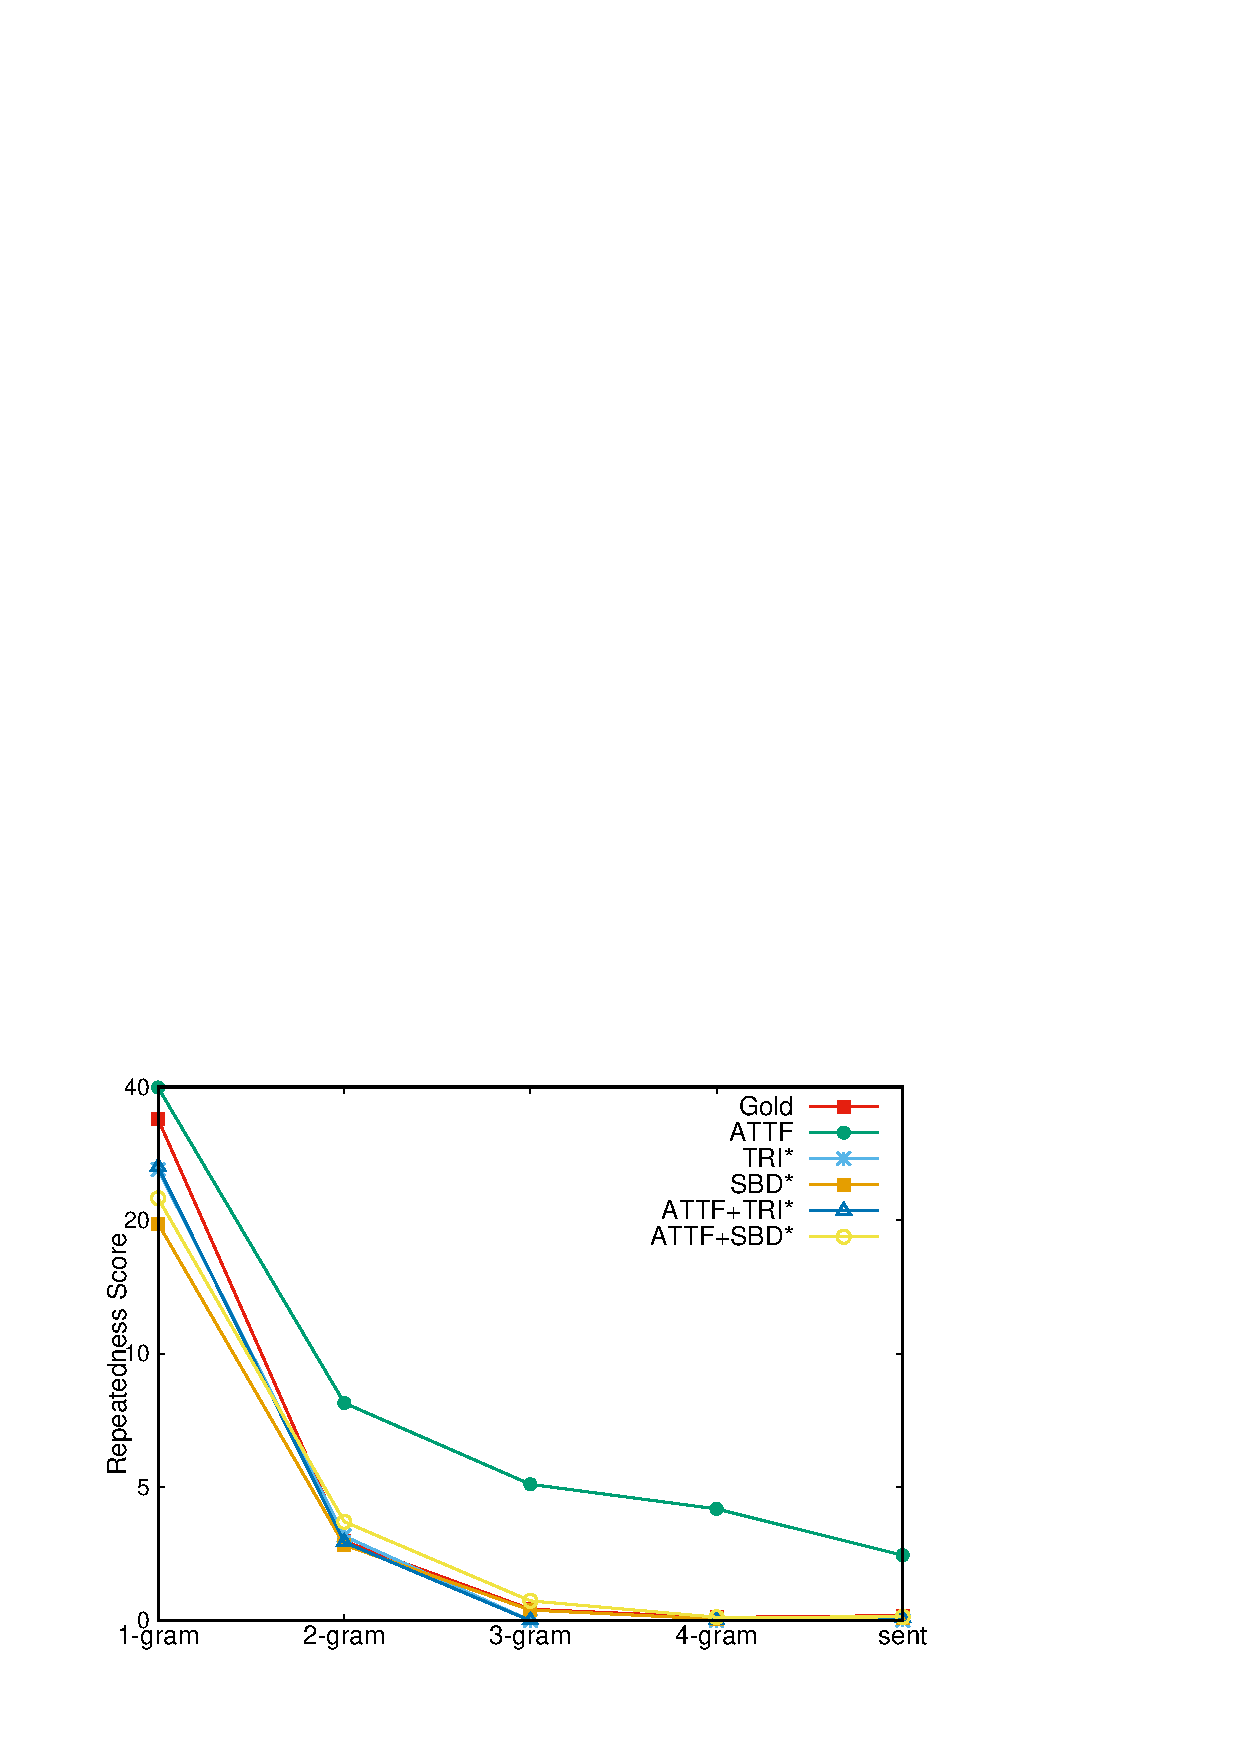
\includegraphics[width=0.9\linewidth]{repeat}
\caption{Repeatedness correlation between generated summaries and Gold summaries.}
\label{fig:repcor}
\end{figure}
}%%%%%%%%%%%


%\KZ{Why do you put total repeatness together with readibility in table 8?
%Why not put it in table 5?}
\cut{%%%%%%%%
\begin{table*}[th]
	\centering
	\scriptsize
	\begin{tabular}{|c|c|c|c|c|c|c|c|c|c|c|}
		\hline
	            & Gold & CNN  & ITA & ITDA & COV & TRI & SBD & ATTF & ATTF+TRI & ATTF+SBD \\
		\hline
		Total-Rep (\%) & 0.51 & 18.86 & 17.94 & 15.62 & 16.46 & \bf 0.0 & 0.44 & 3.27 & \bf 0.0 & 0.80 \\
		Readable & 1.0 & 0.65 & 0.75 & 0.76 & 0.80 & 0.75 & 0.85 & 0.86 & 0.77 & \bf 0.93 \\
		\hline
	\end{tabular}
	\caption{Total Repeatedness and Readability scores on CNN/Daily Mail dataset}
	\label{tab:eval_cor}
\end{table*}
}%%%%%%%%%


\textbf{Readability.}
%Summaries generated by TRI always contain grammatical errors
%and factual errors, such as the TRI row in \tabref{tab:strong_methods}.
%In order to solve it, we proposed correctness(\secref{sec:expset}) as
%one of our evaluation metrics. 
The readability scores of generated summaries are 
shown in \tabref{tab:eval_repe}.
ATTF achieves the
highest readability score among all baselines without 
any operations during testing.
TRI achieves the best score on repeatedness, 
% which represents the repetition over N-gram and sentences,
but lower readability score than other models.
Also, the readability of ATTF drops after adding TRI.
%All of our models score higher than $0.80$. 
SBD enhances performance of CNN and ATTF by reducing the repetitive unreadable sentences. 
ATTF+SBD scores highest on readability.
%\KW{not clear enough}

\begin{table}[th]
\centering
\scriptsize
\begin{tabular}{|l|c|c|c|}
\hline
Model & Time (s) & summaries/s & tokens/s \\
\hline
RNN  &  21600 & 0.48 & 29.60 \\
FastRNN &  3600 & 2.92 & 219.60 \\
\hline
CNN &  346.1 & 30.36 & 1343.46 \\
SBD-b1 &  412.8 & 25.46 & 1126.38 \\
SBD-b2 &  843.5 & 12.16 & 551.24 \\
SBD &  912.8 & 11.51 & 493.68 \\
ATTF & 1332 & 7.89 &  349.00 \\
ATTF+SBD & 1832.3 & 5.74 &  253.77 \\
\hline
\end{tabular}
\caption{Testing time and speed of generation.}
\label{tab:eval_speed}
\end{table}


\textbf{Speed.} 
As shown in \tabref{tab:eval_main} and \tabref{tab:eval_speed}, 
SBD is the best sentence-level backtracking decoder.
Compared with SBD-b1 and SBD-b2,
SBD logs higher ROUGE score without losing much on speed. 
We compare the speed of our model to two RNN 
seq2seq models (RNN and FastRNN)~\cite{SeeLM17, P18-1063}
which used GPU K40. 
%The input and output of RNN seq2seq in this model 
%are both a single sentence, while our model deals with
%multi-sentence sequences simultaneously. 
We perform experiments on GTX-1080ti and scale the speed 
reported for the RNN methods,
since GTX-1080ti is twice as fast as K40~\cite{gehring2017convs2s}.
Our convolutional seq2seq model can 
generate summaries much faster than previous RNN seq2seq models.
%FastRNN is also fast because 

\cut{%%%%%%%%%%%%%%%%%%%
\begin{table*}[th]
	\centering
	\scriptsize
	\begin{tabular}{l|c|c|c|c|c|c|c|c}
		\hline
		Model &   1-gram  & 2-gram & 3-gram & 4-gram & 5-gram & sent & total & Readable \\
		\hline
		Gold & \bf 33.79 & \bf 2.98 & \bf 0.43 & \bf 0.12 & \bf 0.04 & \bf 0.19 & \bf 0.51 & - \\
		\hline
		CNN &  56.25 & 36.55 & 32.62 & 30.18 & 28.07  & 24.13 & 18.86 & 0.65 \\
		ITA & 54.44 & 34.76 &31.10 & 28.85 & 26.89 & 23.15 & 17.94 & 0.75 \\
		ITDA & 51.18 & 30.64 & 27.14 & 25.04 & 23.22 & 20.19 & 15.62 & 0.76 \\
		COV & 42.18 & 16.77 & 12.95 &  & 24.63 & 21.40 & 16.46 & 0.80 \\
		ATTF & 34.98 & 8.16 & 5.11 & 4.19 & 3.65 & 2.45 & 3.27 & 0.86\\
		\hline
		TRI* & 31.91 & 3.17 & - & - & - & 0.01 & - & 0.75 \\
		SBD* & 29.88 & 2.84 & 0.40 & 0.06 & 0.01 & 0.10 & 0.44 & 0.85 \\
		\hline
		ATTF+TRI & 32.0 & 2.94 & - & - & - & 0.09 & - & 0.77 \\
		ATTF+SBD & 30.83 & 3.71 & 0.74 & 0.13 & 0.02 & 0.14  & 0.8 & 0.93 \\
		\hline
	\end{tabular}
	\caption{Repeatedness and Readability scores on CNN/Daily Mail dataset}
	\label{tab:eval_repe}
\end{table*}
}%%%%%%%%%%%%%%%%%%%


